\documentclass{standalone}
\usepackage{tikz}
\usetikzlibrary{patterns, positioning}
\usepackage[sfdefault]{ClearSans} %% option 'sfdefault' activates Clear Sans as the default text font
\usepackage[T1]{fontenc}

\begin{document}
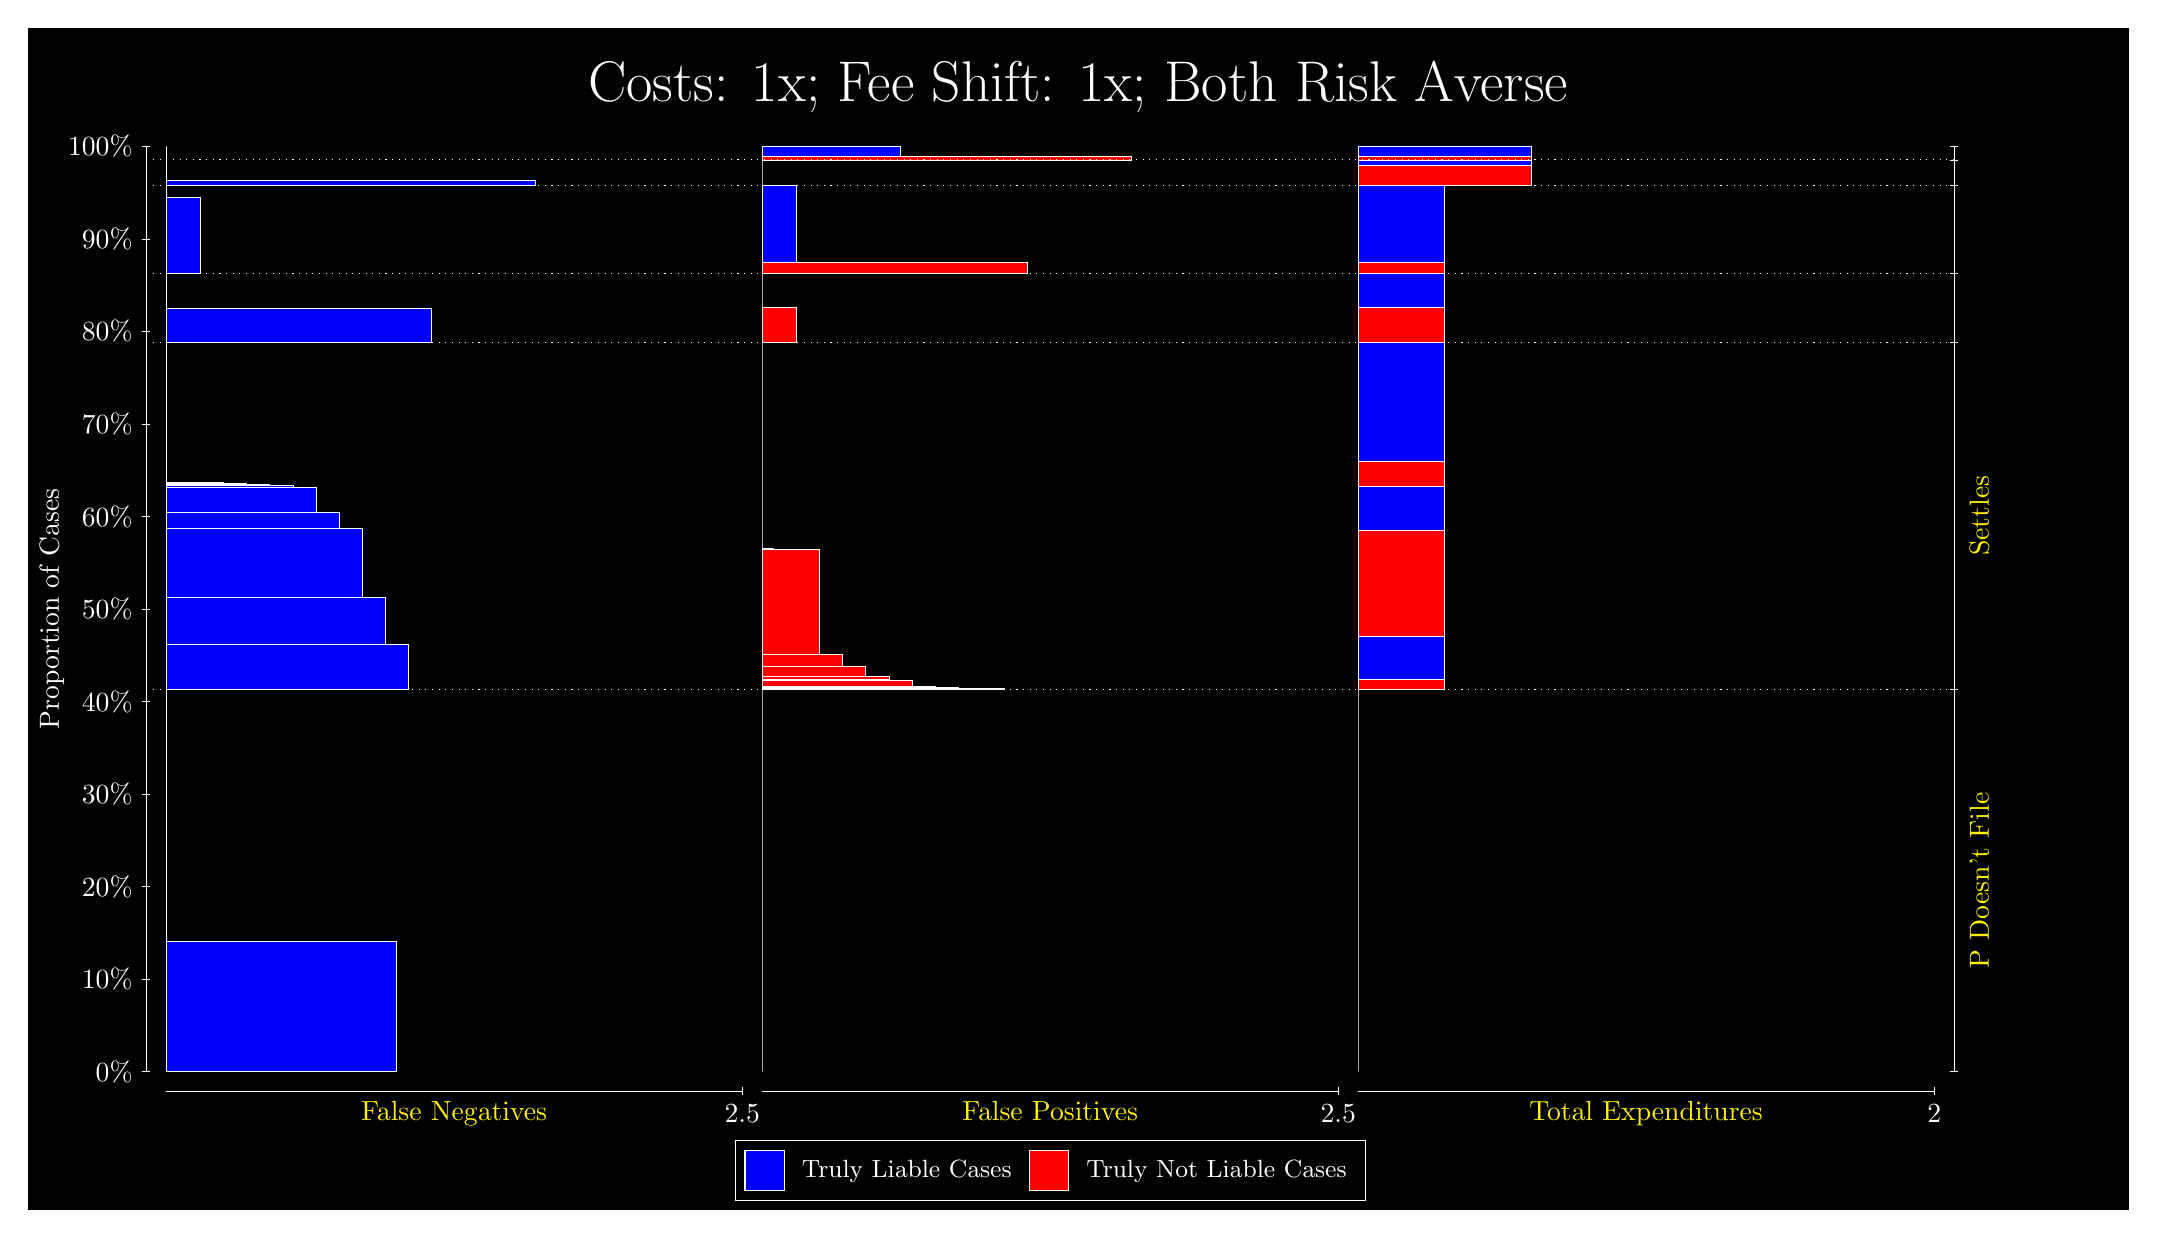
\begin{tikzpicture}
\draw[fill=black] (0,0) rectangle (26.667,15);
\draw[text=white] (0,13.5) rectangle (26.667,15) node[midway] {\huge Costs: 1x; Fee Shift: 1x; Both Risk Averse};
\draw[white, very thin] (1.5,1.75) -- (1.5,13.5);
\node[rotate=90, text=white, anchor=center] at (0.3, 7.625) {Proportion of Cases};
\draw[white, very thin] (1.45,1.75) -- (1.55,1.75);
\node[text=white, anchor=east] at (1.45, 1.75) {0\%};
\draw[white, very thin] (1.45,2.925) -- (1.55,2.925);
\node[text=white, anchor=east] at (1.45, 2.925) {10\%};
\draw[white, very thin] (1.45,4.1) -- (1.55,4.1);
\node[text=white, anchor=east] at (1.45, 4.1) {20\%};
\draw[white, very thin] (1.45,5.275) -- (1.55,5.275);
\node[text=white, anchor=east] at (1.45, 5.275) {30\%};
\draw[white, very thin] (1.45,6.45) -- (1.55,6.45);
\node[text=white, anchor=east] at (1.45, 6.45) {40\%};
\draw[white, very thin] (1.45,7.625) -- (1.55,7.625);
\node[text=white, anchor=east] at (1.45, 7.625) {50\%};
\draw[white, very thin] (1.45,8.8) -- (1.55,8.8);
\node[text=white, anchor=east] at (1.45, 8.8) {60\%};
\draw[white, very thin] (1.45,9.975) -- (1.55,9.975);
\node[text=white, anchor=east] at (1.45, 9.975) {70\%};
\draw[white, very thin] (1.45,11.15) -- (1.55,11.15);
\node[text=white, anchor=east] at (1.45, 11.15) {80\%};
\draw[white, very thin] (1.45,12.325) -- (1.55,12.325);
\node[text=white, anchor=east] at (1.45, 12.325) {90\%};
\draw[white, very thin] (1.45,13.5) -- (1.55,13.5);
\node[text=white, anchor=east] at (1.45, 13.5) {100\%};

\draw[white, very thin] (24.457,1.75) -- (24.457,13.5);
\draw[white, very thin] (24.407,1.75) -- (24.507,1.75);
\node[anchor=west] at (24.407, 1.75) {};
\draw[white, very thin] (24.407,6.606) -- (24.507,6.606);
\node[anchor=west] at (24.407, 6.606) {};
\draw[white, very thin] (24.407,11.013) -- (24.507,11.013);
\node[anchor=west] at (24.407, 11.013) {};
\draw[white, very thin] (24.407,11.889) -- (24.507,11.889);
\node[anchor=west] at (24.407, 11.889) {};
\draw[white, very thin] (24.407,13.001) -- (24.507,13.001);
\node[anchor=west] at (24.407, 13.001) {};
\draw[white, very thin] (24.407,13.327) -- (24.507,13.327);
\node[anchor=west] at (24.407, 13.327) {};
\draw[white, very thin] (24.407,13.5) -- (24.507,13.5);
\node[anchor=west] at (24.407, 13.5) {};

\draw[white, very thin, fill=blue] (1.75,1.75) rectangle (4.6775,3.4104);
\draw[white, very thin, fill=red] (1.75,3.4104) rectangle (1.75,6.606);
\draw[white, very thin, fill=blue] (1.75,6.606) rectangle (4.8239,7.1739);
\draw[white, very thin, fill=blue] (1.75,7.1739) rectangle (4.5312,7.7763);
\draw[white, very thin, fill=blue] (1.75,7.7763) rectangle (4.2384,8.647);
\draw[white, very thin, fill=blue] (1.75,8.647) rectangle (3.9457,8.8553);
\draw[white, very thin, fill=blue] (1.75,8.8553) rectangle (3.6529,9.1744);
\draw[white, very thin, fill=blue] (1.75,9.1744) rectangle (3.3602,9.1929);
\draw[white, very thin, fill=blue] (1.75,9.1929) rectangle (3.0674,9.2128);
\draw[white, very thin, fill=blue] (1.75,9.2128) rectangle (2.7746,9.2221);
\draw[white, very thin, fill=blue] (1.75,9.2221) rectangle (2.4819,9.2327);
\draw[white, very thin, fill=red] (1.75,9.2327) rectangle (1.75,11.013);
\draw[white, very thin, fill=blue] (1.75,11.013) rectangle (5.1167,11.446);
\draw[white, very thin, fill=red] (1.75,11.446) rectangle (1.75,11.889);
\draw[white, very thin, fill=blue] (1.75,11.889) rectangle (2.1891,12.858);
\draw[white, very thin, fill=red] (1.75,12.858) rectangle (1.75,13.001);
\draw[white, very thin, fill=blue] (1.75,13.001) rectangle (6.4341,13.064);
\draw[white, very thin, fill=red] (1.75,13.064) rectangle (1.75,13.327);
\draw[white, very thin, fill=red] (1.75,13.327) rectangle (1.75,13.377);
\draw[white, very thin, fill=blue] (1.75,13.377) rectangle (1.75,13.5);
\draw[white, very thin, fill=red] (9.3189,1.75) rectangle (9.3189,4.9456);
\draw[white, very thin, fill=blue] (9.3189,4.9456) rectangle (9.3189,6.606);
\draw[white, very thin, fill=red] (9.3189,6.606) rectangle (12.393,6.6127);
\draw[white, very thin, fill=red] (9.3189,6.6127) rectangle (12.1,6.6187);
\draw[white, very thin, fill=red] (9.3189,6.6187) rectangle (11.807,6.6313);
\draw[white, very thin, fill=red] (9.3189,6.6313) rectangle (11.515,6.6436);
\draw[white, very thin, fill=red] (9.3189,6.6436) rectangle (11.222,6.7128);
\draw[white, very thin, fill=red] (9.3189,6.7128) rectangle (10.929,6.7343);
\draw[white, very thin, fill=red] (9.3189,6.7343) rectangle (10.929,6.7664);
\draw[white, very thin, fill=red] (9.3189,6.7664) rectangle (10.636,6.9026);
\draw[white, very thin, fill=red] (9.3189,6.9026) rectangle (10.344,7.0467);
\draw[white, very thin, fill=red] (9.3189,7.0467) rectangle (10.051,8.3863);
\draw[white, very thin, fill=blue] (9.3189,8.3863) rectangle (9.4652,8.3968);
\draw[white, very thin, fill=blue] (9.3189,8.3968) rectangle (9.3189,11.013);
\draw[white, very thin, fill=red] (9.3189,11.013) rectangle (9.758,11.456);
\draw[white, very thin, fill=blue] (9.3189,11.456) rectangle (9.3189,11.889);
\draw[white, very thin, fill=red] (9.3189,11.889) rectangle (12.686,12.033);
\draw[white, very thin, fill=blue] (9.3189,12.033) rectangle (9.758,13.001);
\draw[white, very thin, fill=red] (9.3189,13.001) rectangle (9.3189,13.265);
\draw[white, very thin, fill=blue] (9.3189,13.265) rectangle (9.3189,13.327);
\draw[white, very thin, fill=red] (9.3189,13.327) rectangle (14.003,13.377);
\draw[white, very thin, fill=blue] (9.3189,13.377) rectangle (11.075,13.5);
\draw[white, very thin, fill=red] (16.888,1.75) rectangle (16.888,4.9456);
\draw[white, very thin, fill=blue] (16.888,4.9456) rectangle (16.888,6.606);
\draw[white, very thin, fill=red] (16.888,6.606) rectangle (17.986,6.7343);
\draw[white, very thin, fill=blue] (16.888,6.7343) rectangle (17.986,7.2786);
\draw[white, very thin, fill=red] (16.888,7.2786) rectangle (17.986,8.6182);
\draw[white, very thin, fill=blue] (16.888,8.6182) rectangle (17.986,9.186);
\draw[white, very thin, fill=red] (16.888,9.186) rectangle (17.986,9.4985);
\draw[white, very thin, fill=blue] (16.888,9.4985) rectangle (17.986,11.013);
\draw[white, very thin, fill=red] (16.888,11.013) rectangle (17.986,11.456);
\draw[white, very thin, fill=blue] (16.888,11.456) rectangle (17.986,11.889);
\draw[white, very thin, fill=red] (16.888,11.889) rectangle (17.986,12.033);
\draw[white, very thin, fill=blue] (16.888,12.033) rectangle (17.986,13.001);
\draw[white, very thin, fill=red] (16.888,13.001) rectangle (19.083,13.265);
\draw[white, very thin, fill=blue] (16.888,13.265) rectangle (19.083,13.327);
\draw[white, very thin, fill=red] (16.888,13.327) rectangle (19.083,13.377);
\draw[white, very thin, fill=blue] (16.888,13.377) rectangle (19.083,13.5);
\draw[white, dotted] (1.5,6.606) -- (24.457,6.606);
\draw[white, dotted] (1.5,11.013) -- (24.457,11.013);
\draw[white, dotted] (1.5,11.889) -- (24.457,11.889);
\draw[white, dotted] (1.5,13.001) -- (24.457,13.001);
\draw[white, dotted] (1.5,13.327) -- (24.457,13.327);
\draw[white, very thin] (1.75,1.5) -- (9.0689,1.5);
\node[text=yellow, anchor=north] at (5.4094, 1.5) {False Negatives};
\draw[white, very thin] (9.0689,1.45) -- (9.0689,1.55);
\node[text=white, anchor=north] at (9.0689, 1.45) {2.5};

\draw[white, very thin] (9.3189,1.5) -- (16.638,1.5);
\node[text=yellow, anchor=north] at (12.978, 1.5) {False Positives};
\draw[white, very thin] (16.638,1.45) -- (16.638,1.55);
\node[text=white, anchor=north] at (16.638, 1.45) {2.5};

\draw[white, very thin] (16.888,1.5) -- (24.207,1.5);
\node[text=yellow, anchor=north] at (20.547, 1.5) {Total Expenditures};
\draw[white, very thin] (24.207,1.45) -- (24.207,1.55);
\node[text=white, anchor=north] at (24.207, 1.45) {2};

\node[text=yellow, centered, rotate=90] at (24.777, 4.178) {P Doesn't File};
\node[text=yellow, centered, rotate=90] at (24.777, 8.8095) {Settles};





\draw (12.978300999999998,1.5) node[draw=none] (baseCoordinate) {};
\begin{scope}[align=center]
        \matrix[scale=0.5, draw=white, below=0.5cm of baseCoordinate, nodes={draw}, column sep=0.1cm]{
            \node[rectangle, draw, minimum width=0.5cm, minimum height=0.5cm, fill=blue] {}; &
            \node[draw=none, font=\small, text=white] (B) {Truly Liable Cases}; &
            \node[rectangle, draw, minimum width=0.5cm, minimum height=0.5cm, fill=red] {}; &
            \node[draw=none, font=\small, text=white] (B) {Truly Not Liable Cases}; \\
            };
\end{scope}

\end{tikzpicture}
\end{document}